\chapter{Schroedinger equation in 3d}

After we have considered two-dimensional Schroedinger equations, we are now ready for
the extension to three-dimensional systems. In 3d, Schroedinger equation can be
written as:
\begin{equation}
\left[ -\frac{1}{2}\nabla^2 + V(\mathbf{r}) \right] \psi(\mathbf{r}) = E\,\psi(\mathbf{r})
\end{equation}
where $\mathbf{r}$ is the abbreviation to $(x,y,z)$ and
%
$\nabla^2$ is the Laplacian operator in 3d:
\begin{equation}
\nabla^2 = \frac{\partial^2}{\partial x^2} + \frac{\partial^2}{\partial y^2} +
\frac{\partial^2}{\partial z^2}
\end{equation}

\subsection{Three-dimensional grid}

As in the preceeding chapter, our first task is to create a representation of 3d grid
points and various quantities defined on it. This task is realized using straightforward
extension of \txtinline{FD2dGrid} to \txtinline{FD3dGrid}.


Visualization of 3d functions as isosurface map or slice of 3d array.

Introducing 3d xsf


\subsection{Laplacian operator}

\begin{equation}
\mathbb{L} = \mathbb{D}^{(2)}_{x} \otimes \mathbb{I}_{y} \otimes \mathbb{I}_{z} +
\mathbb{I}_{x} \otimes \mathbb{D}^{(2)}_{y} \otimes \mathbb{I}_{z} +
\mathbb{I}_{x} \otimes \mathbb{I}_{y} \otimes \mathbb{D}^{(2)}_{z}
\end{equation}


Code
\begin{juliacode}
const ⊗ = kron
function build_nabla2_matrix( fdgrid::FD3dGrid; func_1d=build_D2_matrix_3pt )
    D2x = func_1d(fdgrid.Nx, fdgrid.hx)
    D2y = func_1d(fdgrid.Ny, fdgrid.hy)
    D2z = func_1d(fdgrid.Nz, fdgrid.hz)
    IIx = speye(fdgrid.Nx)
    IIy = speye(fdgrid.Ny)
    IIz = speye(fdgrid.Nz)
    ∇2 = D2x⊗IIy⊗IIz + IIx⊗D2y⊗IIz + IIx⊗IIy⊗D2z 
    return ∇2
end
\end{juliacode}

The main difference is that we have used the symbol \txtinline{⊗} in place
of \txtinline{kron} function to make our code simpler.


\section{3d harmonic oscillator}

We hope that at this point you will have no difficulties to create your own
3d Schroedinger equation solver.

Analytic solution for energy:
\begin{equation}
E_{n_{x} + n_{y} + n_{z}} = \hbar \omega \left( n_{x} + n_{y} + n_{z} + \frac{3}{2} \right)
\end{equation}

Degeneracies:
\begin{equation}
g_{n} = \frac{(n + 1)(n + 2)}{2}
\end{equation}

\begin{textcode}
n = n_x + n_y + n_z

n = 0: (1)(2)/2 = 1
n = 1: (2)(3)/2 = 3
n = 2: (3)(4)/2 = 6
\end{textcode}


\section{Hydrogen atom and an introduction to pseudopotential}

Until now, we only have considered simple potentials such as harmonic potential. Now we will
move on and consider more realistic potentials which is used in practical electronic calculations.

For most applications in materials physics and chemistry the external potential that is
felt by electrons is the Coulombic potential due to atomic nucleus. This potential has
the following form:
\begin{equation}
V(r) = -\sum_{I}^{N_{\mathrm{atom}}} \frac{Z_{I}}{\left|\mathbf{r} - \mathbf{R}_{I}\right|}
\end{equation}
where $R_{I}$ are the positions and $Z_{I}$ are the charges
of the atomic nucleus present in the system.
%
We will consider the most simplest system, namely the hydrogen atom $Z_{I}=1$, for which we have
\begin{equation}
V(r) = -\frac{1}{\left|\mathbf{r} - \mathbf{R}_{0}\right|}
\end{equation}
%
The following Julia code implement the H atom potential:
\begin{juliacode}
function pot_H_atom( fdgrid::FD3dGrid; r0=(0.0, 0.0, 0.0) )
    Npoints = fdgrid.Npoints
    Vpot = zeros(Npoints)
    for i in 1:Npoints
        dx = fdgrid.r[1,i] - r0[1]
        dy = fdgrid.r[2,i] - r0[2]
        dz = fdgrid.r[3,i] - r0[3]
        Vpot[i] = -1.0/sqrt(dx^2 + dy^2 + dz^2)
    end
    return Vpot
end
\end{juliacode}

With only minor modification to our program for harmonic potential, we can solve the Schroedinger
equation for the hydrogen atom:
\begin{juliacode}
fdgrid = FD3dGrid( (-5.0,5.0), Nx, (-5.0,5.0), Ny, (-5.0,5.0), Nz )
∇2 = build_nabla2_matrix( fdgrid, func_1d=build_D2_matrix_9pt )
Vpot = pot_H_atom( fdgrid )
Ham = -0.5*∇2 + spdiagm( 0 => Vpot )
prec = aspreconditioner(ruge_stuben(Ham))
Nstates = 1  # only choose the lowest lying state
Npoints = Nx*Ny*Nz
X = ortho_sqrt( rand(Float64, Npoints, Nstates) ) # random initial guess of wave function
evals = diag_LOBPCG!( Ham, X, prec, verbose=true )
\end{juliacode}

For the grid size of $N_{x}=N_{y}=N_{z}=50$ and using 9-point finite-difference approximation
to the second derivative operator in 1d we obtain the eigenvalue of -0.4900670759 Ha which
is not too bad if compared with the exact value of -0.5 Ha. We can try to increase the grid
size until we can get satisfactory result.

Note that there is a caveat when we are trying to use the Coulombic potential. This potential
is diverget at $r=0$, so care must be taken such that this divergence is not encountered in
our potential. We have tried to achieve this by using choosing the numbers
$N_{x}$, $N_{y}$, and $N_{z}$ to be even numbers. This way, we have avoiding encountering
divergence in the calculation of Coulomb potential.

In the many electronic structure calculations, it is sometime convenient to replace the
Coulomb potential with another potential which is smoother which we
will refer to as a \textbf{pseudopotential}. Not all smooth
potentials can do the job. The smooth potential should satisfy several requirements.
One of the most important requirement is that the smooth potential should have similar
scattering properties as the original Coulomb potential that it replaces.
This means that the potential should have posses similar eigenvalues as the
original Coulomb potential. Usually we don't try to reproduce all eigenvalue spectrum but only
the eigenvalues which belongs to the valence electrons. The valence electrons are
responsible for most chemically and physically important properties so this is an
acceptable approximation for most cases.

The theory and algorithms for constructing pseudopotentials are beyond the scope of
this article.
Most pseudopotentials are non-local by construction and this can make our program rather
complicated.
In this article we focus on the so-called local pseudopotential. Practically, local
pseudopotentials pose no additional difficulties as the potentials that we have
considered so far. As an example of a pseudopotential, we will consider the following
local pseudopotential for hydrogen atom:
\begin{equation}
V_{\mathrm{H,ps}}(r) = -\frac{Z_{\mathrm{val}}}{r}
\mathrm{erf}\left( \frac{\bar{r}}{\sqrt{2}} \right) +
\exp\left( -\frac{1}{2}\bar{r}^2 \right)
\left( C_{1} + C_{2}\bar{r}^2 \right)
\end{equation}
where $\bar{r}=r/r_{\mathrm{loc}}$ and with the parameters $r_{loc}=0.2$, 
$Z_{\mathrm{val}}=1$, $C_{1}=-4.0663326$, and $C_{2}=0.6678322$.

\begin{figure}[H]
{\centering
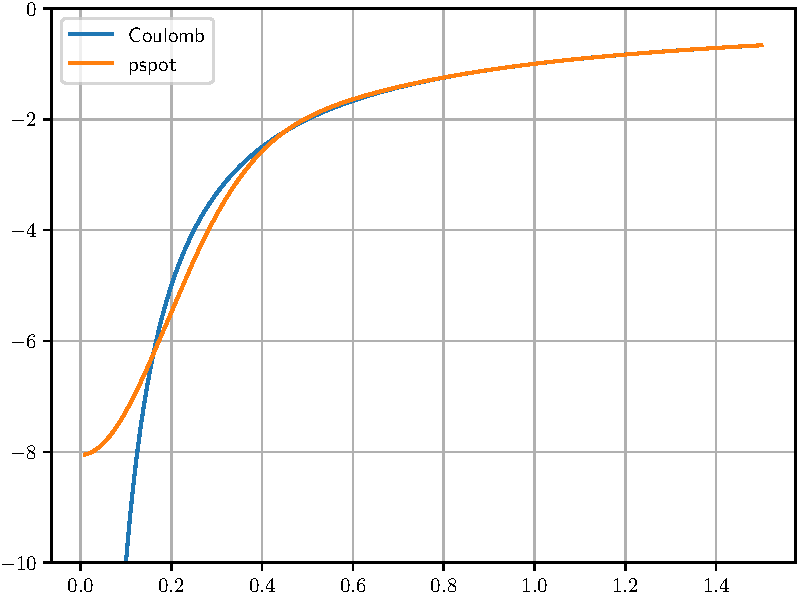
\includegraphics[width=0.65\textwidth]{../codes/sch_3d/IMG_H_Coulomb_vs_pspot.pdf}
\par}
\caption{Comparison Coulomb potential vs pseudopotential}
\end{figure}

The code
\begin{juliacode}
function pot_Hps_HGH( fdgrid::FD3dGrid; r0=(0.0, 0.0, 0.0) )
    Npoints = fdgrid.Npoints
    Vpot = zeros( Float64, Npoints )

    # Parameters
    Zval = 1
    rloc = 0.2
    C1 = -4.0663326
    C2 = 0.6678322
    for ip = 1:Npoints
        dx2 = ( fdgrid.r[1,ip] - r0[1] )^2
        dy2 = ( fdgrid.r[2,ip] - r0[2] )^2
        dz2 = ( fdgrid.r[3,ip] - r0[3] )^2
        r = sqrt(dx2 + dy2 + dz2)
        if r < eps()
            Vpot[ip] = -2*Zval/(sqrt(2*pi)*rloc) + C1
        else
            rrloc = r/rloc
            Vpot[ip] = -Zval/r * erf( r/(sqrt(2.0)*rloc) ) +
                     (C1 + C2*rrloc^2)*exp(-0.5*(rrloc)^2)
        end
    end
    return Vpot
end
\end{juliacode}
